\documentclass[10pt]{jreport}
%
%%%% 文中の欧文をPSフォントにするならコメントアウトを外す
%\usepackage{times}
%\usepackage[T1]{fontenc}
%\normalfont
%\usepackage{mathptm}
%
%%%% M2ならbachelorをmasterにする
\usepackage{sty/master}
\usepackage{sty/rsfs}
\usepackage{float}
%
%
%%%% dvipdfmなどを使うならuseDVIPDFMtrueにする
\newif\ifuseDVIPDFM\useDVIPDFMfalse
%
%%%% hyperrefを使うとpdf中にハイパーリンクが作れるが,しおりなどがちゃん
%%%% とできるようにするためには,W32TeXで有名な角藤さんが作られたout2uni
%%%% (dvipdfmxの場合)やbkmk2uni (dvipsk,pdvipsを使う場合)を使う必要があ
%%%% る(W32TeXでは使える.suzakuでも使用可能)
\usepackage[dvipdfmx]{graphicx}

%

%
%%%% 図のhlineを太さ指定可能にするための呪文
%%%% (\bhline{1.0pt}という感じで使用)
\newcommand{\bhline}[1]{\noalign{\hrule height #1}}
%

%
%%%% 図の位置調整をより強力に行うための呪文
%%%% (\begin{figure}[H]という感じで使用)
\floatstyle{plain}
\newfloat{myalgo}{tbhp}{mya}
\newenvironment{Algorithm}[2][tbh]%
{\begin{myalgo}[#1]
\centering
\begin{minipage}{#2}
\begin{algorithm}[H]}%
{\end{algorithm}
\end{minipage}
\end{myalgo}}
%
%
%キャプション再定義
%
%
%%%% その他,諸々の必要なもの
\usepackage{amsmath,amssymb}
\usepackage{url}
\usepackage{sty/jdummy}
\usepackage{mediabb}
\usepackage{sty/algorithm}
\usepackage{sty/algorithmic}
\usepackage{subcaption}
\usepackage{bm}
\usepackage[dvipdfmx]{color}
\usepackage{subcaption}
\captionsetup[sub]{margin=5pt}
%
%
%マクロ再定義
%
%
% キャプションをすべてゴシック体に変更
\makeatletter

\long\def\@makecaption#1#2{
  \advance\leftskip1cm
  \advance\rightskip1cm
  \vskip\abovecaptionskip
  \sbox\@tempboxa{{\bf #1}\hskip1zw{\gt #2}}%
  \ifdim \wd\@tempboxa >\hsize
    {\bf #1}\hskip1zw{\gt #2}\par
  \else
    \global \@minipagefalse
    \hb@xt@\hsize{\hfil\box\@tempboxa\hfil}%
  \fi
  \vskip\belowcaptionskip}

\makeatother
%
% subcaptionで定義した場合の子ラベルを読み込んでくれるマクロ.
% \subfigref{図のキャプション}{サブキャプション}で図1(a)のように出力.
\def\subfigref#1#2{\textgt{図\,\ref{#1}(\subref{#2})}}
\definecolor{legend1}{rgb}{1.00,0.00,0.00}
\definecolor{legend2}{rgb}{0.99,0.65,0.40}
\definecolor{legend3}{rgb}{0.87,0.87,0.87}
\definecolor{legend4}{rgb}{0.66,0.54,1.00}
\definecolor{legend5}{rgb}{0.40,0.18,1.00}
%
%
%
%
%\usepackage[dvipdfmx]{hyperref}
%\usepackage{pxjahyper}
%
\begin{document}
	
\title{音源に同期する運指および表情に注目した\\
	吹奏アニメーションの自動生成}
\author{堀井 絵里}
%%%% masterの場合,次の3行は無効
\teacher{藤代 一成}
\id{81621728}
\date{\the\year 年2月5日}

%%%% 回答書(最終提出版では削除)
\iftrue
%\iffalse
\pagestyle{empty}
%%%%%%%%%%%%%%%%%%%%%%%%%%%%%%%%%%%%%%%%%%
%%%%%%%% �������� %%%%%%%%%%%%%%%%%%%%%%%%
%%%% �K�v�������L�������������D
%% �񓚏���o��
\newcommand\submisson{����28�N1��22��}
%% ����
\newcommand\affiliation{�c��`�m��w ���H�w������\\
�J���‹��Ȋw��U ���H�w��C}
%% �_���^�C�g��
\newcommand\thesistitle{�����ɓ�������^�w����ѕ\��ɒ��ڂ������t�A�j���[�V�����̎�������}
%% �w�Дԍ�
\newcommand\studentid{81621728}
%% ���O
\newcommand\myname{�x�� �G��}
%%%%%%% �����܂ł� %%%%%%%%%%%%%%%%%%%%%
%%%%%%%%%%%%%%%%%%%%%%%%%%%%%%%%%%%%%%%%%%


%%%% �ȉ��񓚏�1���ڏ���
{\large
\begin{flushright}
\submisson
\end{flushright}
\noindent
\affiliation\ �䒆
}
\vspace{2cm}
{\LARGE
\begin{center}
�C�m�_�����\�ɂ����鎿��ɑ΂���񓚕�
\end{center}
}
\vspace{2cm}
{\Large
\noindent
���Ҋw�Дԍ��F\studentid
\\
��ځF\\
\thesistitle
}

\vspace{1.5cm}
{\large 
\noindent
�q�[\\
�����܂��܂������˂̂��ƂƂ��c�ѐ\���グ�܂��D\\
���̓x�́C���̏C�m�_�����\�ɂ����ċM�d�ȃR�����g������܂��Đ��ɂ��肪�Ƃ��������܂����D���Ղ����R�����g�ɏ]���C�ȉ��̂悤�ȕ��j�Ɋ�Â��ĉ��ǂ������܂����̂ŁC���m�F��������낵�����肢�\���グ�܂��D
\begin{flushright}
�h��\\
\myname
\end{flushright}
}
\newpage

\newenvironment{qanda}
{\begin{enumerate}
\def\theenumi{\bf{\underline{����\arabic{enumi}}}}
\def\labelenumi{\theenumi}
\let\escapeitem\item
\renewcommand\item{\setlength{\parskip}{0.5cm} \escapeitem}
}
{\end{enumerate}
\def\labelenumi{\arabic{enumi}.}
\let\item\escapeitem
}
\newcommand\q[1]{\textbf{\underline{#1}}\\}

\begin{qanda}
%%%%%%%%%%%%%%%%%%%%%%%%%%%%%%%%%%%%%%%%%%
%%%%%%%% ��������񓚊J�n %%%%%%%%%%%%%%%
%%%% ����Ɖ񓚂�
%%%% \item \q{question (professer)}\\
%%%% answer...
%%%% �̂悤�ɏ����D
%%%% <<����>> LaTeX�͉����t�����{������s�ł��Ȃ��̂ŁC
%%%% �����Œ��x�ǂ�����\q{aaa}\q{bbb}�Ƌ�؂邱�ƁD

\item \q{�s���R�ȗ�Ƃ��Ď�������`���̃A�j���[�V�����ƁC�����������Ă���3DCG�̃A�j���[�V������}
\q{�{���I�ɈႤ�̂ł͂Ȃ����D�i�֓��p�Y�搶�j}\\
%
�@�‚�ʂ�C�{���͈Ⴂ�܂��D
�������C���ۂ�3DCG�ł��̂悤�ȃV�[�����Č�����ꍇ���C���Ɠ�����1�‚����킹��ɂ͎��ԂƘJ�͂�������Ƃ������Ƃ́C�A�j���[�V��������ɏڂ����҂��畷���Ă���܂��D\\
�@���ۂɁC�{��@�ɂ��A�j���[�V��������̎��Ԃ���јJ�͂̌y���ɂ‚��āC�A�j���[�V��������ɏڂ����҂փA���P�[�g���Ƃ����Ƃ���C���ۂɌy�������Ɨ\�z�����҂��قƂ�ǂł����D���̂��߁C�{��@�ɂ��3DCG�̃A�j���[�V��������̎��Ԃ���јJ�͂̌y�����”\�ł���Ƃ����܂��D
������̃A���P�[�g���ʂ́C{\gt4.2.4��}�Ɏ����Ă���܂��D\\
%%%
%%%
\item \q{���Ǝw�̃��[�V�����͂ǂ̂悤�Ƀ}�b�s���O���Ă���̂��D�i�֓��p�Y�搶�j}\\
%
�@�g�����y�b�g�Ɋւ��ẮC���ꂼ��̎w�̏�Ԃ��C�s�X�g���������������Ȃ�����2�‚ƂȂ�܂��D
����g�����{�[���Ɋւ��ẮC�X���C�h���~�߂�ꏊ��7�ӏ����݂��܂��D
������̊y����C���Ǝw��r�̏�Ԃ�1��1�őΉ������邱�Ƃ��”\�ł��邽�߁C�����ς��Ƃ��̉����‚�悤�Ȏp���ɑJ�ڂ��C��������̒��������ۂC�Ƃ����������ɂȂ��Ă���܂��D\\
�@��L�̓��e�́C{\gt3.8.1��}�ɂďڐ����Ă���܂��D\\
%%%
%%%
\item \q{���NJy�킲�ƂɃ}�b�v�\���쐬���邱�Ƃɂ��C�ǂ̊y��ł������������”\�ł���Ƃ����_��}
\q{�V�K���Ȃ̂��D�i�֓��p�Y�搶�j}\\
%
\indent
�@�͂��C�‚�ʂ�ł��D
�}�b�v�\�ƃ��f����������΁C�ǂ̋��NJy��ł��e�Ղɐ��t�A�j���[�V�����̎����������”\�ƂȂ��Ă���܂��D\\
�@������ɂ‚��ẮC{\gt2.5��}�ɋL�ڂ������܂����D\\
%%%
%%%
\item \q{���y��Ɋg�����鎞�ɉ������K�v�ƂȂ�ۑ�͉����D�i���Y�搶�j}\\
%
�@���y��͋��NJy��Ƃ͈قȂ�\��̕ω��͏������ł����C���ƌ��̉���������1��1�ł͂Ȃ����߁C�ǂ̎w�g�����K�؂Ȃ̂����C����‚炷�x�ɍl������悤�ȏ�����������K�v������܂��D\\
�@���y��̏ꍇ��{\gt2.1��}�ŏЉ�Ă����s���������݂��邽�߁C��������Q�l�Ɏ������s�����Ƃɂ��C�Ή����”\�ł���ƍl�����܂��D\\
%%%
%%%
\newpage
\item \q{�����𐁂�������Ɛh���Ȃ�l�q���C�ċz�̃p�����^��p���ĕ\�����邱�Ƃɂ‚��āD�i���Y�搶�j}\\
%
�@�����܂����A�h�o�C�X�̒ʂ�C��莞�ԑ��p�������Ă��Ȃ��C���邢�͍����悪�����ȂǁC�h���Ȃ�悤�ȏ����𖞂������ۂɐh�����ȕ\�������C�Ƃ��������Ƃ͎������”\�ł��D
������Ɋւ��ẮC���[�V�����Ɋւ��郁�^�f�[�^��p�ӂ��C������ɕ\��⃂�[�V�����̎w����L�ڂ��邱�Ƃ��l���Ă���܂��D
�����I�ɎZ�o�ł���ꍇ�͎Z�o���C�Z�o���ł��Ȃ��ꍇ�͂�����̃f�[�^�ɋL�ڂ��邱�Ƃɂ��C�\�����”\�ł���ƍl�����܂��D\\
�@�\��𐧌䂷�邽�߂ɂ́C���b�V���𐧌䂷��K�v������܂��D
Unreal Engine�Ń��b�V���𐧌䂷��ہC���[�t�^�[�Q�b�g�Ƃ����@�\��p���܂����C���̋@�\�̓u�����h�V�F�C�v���K�p����Ă��Ȃ����b�V���ɂ͎g�p�ł��܂���D
�����ŁC�u�����h�V�F�C�v�Ƃ́C���炩���ߗp�ӂ��ꂽ�����̕\��f�����p�����^�̒����ɂ��g�ݍ��킹�邱�ƂŁC���܂��܂ȕ\����쐬����A�j���[�V������@�������܂��D
����p�������j�e�B�����́C�f�t�H���g�Ō����Ƀu�����h�V�F�C�v���ݒ肳��Ă��邽�߁C���[�t�^�[�Q�b�g�ɂ������̐��䂪�”\�ł��D
�������h���\��Ȃǂ��Č����邽�߂ɂ́C�f�t�H���g�̐ݒ�ł̓u�����h�V�F�C�v���s�����Ă��邽�߁C���̃\�t�g�E�F�A����čĐݒ肷��K�v������ƍl�����܂��D
�‚܂�CUnreal Engine�݂̂ł͍Č����s�”\�ł���Ƃ����܂��D\\
\indent
�@��L�̓��e�ɂ‚��ẮC����̉ۑ�Ƃ���{\gt5.2.1��}�ɂ܂Ƃ߂܂����D\\
%%%
%%%
\item \q{�l�ɂ�铮���̈Ⴂ���e���t�҂ɓK�p������@�ɂ‚��āD�i���{�搶�j}\\
%
�@���ƂȂ郂�[�V�����͑S�ē����ł����C���̃��[�V�����̑傫����0����1�̃p�����^�Ń����_���ɐݒ肷�邱�Ƃɂ��C�l�����o���H�v�����Ă��܂��D
���Y�搶���炲�w�E������܂����C���t�҂��Ƃɑ̌^���قȂ�ꍇ�́C����5�ŏq�ׂ����^�f�[�^�ɂ��̎|���L�ڂ��C���[�V�����𕪂���K�v������ƍl�����܂��D\\
�@�O�҂̓��e�ɂ‚��Ă�{\gt3.8.3��}�ɁC��҂̓��e�ɂ‚��Ă͍���̉ۑ�Ƃ���{\gt5.2.4��}�ɋL�ڂ������܂����D\\
%%%
%%%
\item \q{���j�e�B������Unreal Engine�Ŏg�p���邱�Ƃɂ‚��āD�i���{�搶�j}\\
%
�@���쌠�I�ɂ͖�育�����܂���D
������ɂ‚��Ắw���j�e�B����񃉃C�Z���X�����x�̑�3���ɂĔ��f�ł��܂��D�iURL: http://unity-chan.com/contents/license\_jp/�j\\
�@��L�̓��e�́C{\gt3.6��}�ɖ��L�������܂����D

%%%%%%%% �����܂� %%%%%%%%%%%%%%%%%%%%%%%%
%%%%%%%%%%%%%%%%%%%%%%%%%%%%%%%%%%%%%%%%%%
\end{qanda}

\begin{flushright}
{\large
�ȏ�
}
\end{flushright}

\renewcommand\submisson{\relax}
\renewcommand\affiliation{\relax}
\renewcommand\thesistitle{\relax}
\renewcommand\studentid{\relax}
\renewcommand\myname{\relax}
\renewcommand\q{\relax}

\newpage
\fi

%%%% 表紙
\pagenumbering{Alph}
\thispagestyle{empty}	% ページ数をつけない
% 修士論文記入用フォーマット
%\newgeometry{left=1.0cm,right=1.0cm}
{\LARGE 修士論文} \hspace{\fill} {\LARGE 2017年度}
\vspace{3cm}
\begin{center}
{\LARGE 音源に同期する運指および表情に注目した	吹奏アニメーションの自動生成}
\\
\vspace{2cm}
{\LARGE 堀井 絵里} \\ \vspace{1.5ex}
{\LARGE (学籍番号:81621728)} \\
\vspace{6.5cm}
{\LARGE 指導教員 教授 藤代 一成} \\
\vspace{2.5cm}
{\Large 2018年3月} \\
\vspace{0.8cm}
{\LARGE 慶應義塾大学大学院理工学研究科} \\ \vspace{1.5ex}
{\LARGE 開放環境科学専攻} \\
\end{center}
%\restoregeometry
		% 論文表紙読み込み
\newpage

%%%% アブストラクト
\thispagestyle{empty}
\begin{center}
{\bf {\large 論文要旨}}
\end{center}

\vspace{3ex}
音楽演奏を題材としたアニメーションは多く存在する.
テレビで放映されたアニメーションの例を挙げると,『のだめカンタービレ』,『けいおん!』,『響け!ユーフォニアム』が相当する.
これらのアニメーションは,セル画であったり3DCGであったり,製作方法はさまざまであるが,いずれも実際に演奏する演奏者の身体の動きに近い演奏アニメーションが生成されている.
楽器の輝きや形状なども忠実に再現されている.
%
しかし,楽器を演奏するキャラクタの運指や身体の動きが,音楽に完全に同期されていないことがある.
特に速いフレーズや,複雑なリズムを演奏するシーンで,このようなアーティファクトが起きやすい.
また,表情からも不自然さを感じることがある.
これらの違和感を解消するためには,身体の動きを1つずつ音階やリズムなどに手動で合わせる必要がある.
この方法は効率が悪く,多くの時間と労力が必要となる.\\
%
\indent
上記の課題を解決するため,鍵盤楽器や弦楽器を演奏する演奏者のアニメーションを,音源から自動生成する研究が存在する.
しかし,管楽器を対象とした研究は,我々の知るかぎりでは存在しない.
そこで本研究では,管楽器を演奏するキャラクタの吹奏アニメーションを,音源から自動生成することを目指した.
アニメータの作業支援を目的とするため,自動生成の流れは実際の演奏アニメーション制作フローに沿わせた.
より具体的には,楽曲は電子楽器を用いてMIDI音源として生成する.
次に,作成した楽曲を解析することにより,吹奏の情報を得る.
最後に,得られた情報をキャラクタの身体の動きや表情,そして管楽器に適用することにより,音源に同期した自然な吹奏アニメーションを実現した.
\indent
自動生成したアニメーションについて評価を行った結果,提案手法により,自然なアニメーションを自動的に生成できることを確認した.

\vspace{4ex}

\noindent
\textgt{キーワード}

\noindent
アニメーション,吹奏楽,金管楽器,自動生成.		% 日本語アブストラクト読み込み
\newpage	
\thispagestyle{empty}
\begin{center}
{\bf {\large Thesis Abstract}}

\vspace{2ex}

{\bf {\large Automatic Generation of Blowing Animation Taking Fingering and Expression Synchronized with Digital Music into Account}}
\end{center}

\vspace{3ex}

\parindent 0.4 in
There are known many animation works with the theme of music performance. Representative televised example of these include ``Nodame Cantabile", ``K-ON!", and ``Hibike! Euphonium", all of which commonly aim at generating realistic motion of performers as well as faithfully reproducing the shape and appearance of the instruments though the underlying production method varies from each other. However, the performer's fingering and motions are sometimes not completely synchronized with music, and thus giving a sense of incompatibility. This type of artifact occurs especially in a scene that he/she plays a fast phrase or in a complex rhythm. Also, facial expressions in animation series occasionally look unnatural. In order to eliminate these kinds of discomfort, it is necessary to manually synchronize the movement of the body one by one with the scale, rhythm, and so on. This work is inefficient because tedious work and much effort are required.\par
%
In order to address these issues, there are known works to automatically generate animations of performers playing keyboard instruments and stringed instruments from sound sources. However, to the best of the author's knowledge, there are no previous works targeting at wind instruments. Therefore, in this thesis research, we aimed to automatically generate blowing animation of characters playing wind instruments from sound sources. For the purpose of animator's work assistance, animation was generated in accordance with the actual animation production flow of musical performance. More specifically, the sound source was generated as a MIDI sound source using an electronic musical instrument. Next, we analyzed the generated sound source to obtain music information. Finally, by applying the obtained information to the character's movement, facial expression, and wind instruments, we generated natural blowing animation synchronized with the sound source.\par
%
Evaluation on the resultant animation by third parties empirically proved that the proposed method can generate natural animation automatically.
\vspace{4ex}

\noindent
{\bf Keywords}

\noindent
Animation; wind orchestra; brass instrument; and automatic generation.

\parindent 1zw		% 英語アブストラクト読み込み
\newpage

%%%% 目次
\pagenumbering{roman}           % ローマ数字のページナンバリング
\tableofcontents                % 目次作成
\listoffigures                  % 図一覧作成
\listoftables                   % 表一覧作成
\newpage
\pagenumbering{arabic}          % アラビア数字のページナンバリング

%%%% はじめに
\chapter{序論}
\label{chap:intro}

本章では,本研究の研究背景と研究目的について説明する.
\secref{sec:background}で研究背景,
\secref{sec:purpose}で研究目的,
\secref{sec:structure}で本論文の構成について述べる.

\section{研究背景}\label{sec:background}
\indent
音楽演奏を題材としたアニメーションは多く存在する.
テレビで放映されたアニメーションの例を挙げると,『のだめカンタービレ』,『けいおん!』,『響け!ユーフォニアム』が相当する.
これらのアニメーションは,セル画であったり3DCGであったり,製作方法がさまざまであるが,いずれも実際に演奏する演奏者の身体の動きに近い演奏アニメーションが生成されている.
楽器の輝きや形状なども忠実に再現されている.
しかし,楽器を演奏するキャラクタの運指や身体の動きに注目すると,音楽と動きが完全に同期されていないことがあり,違和感を感じる.
特に速いフレーズや,複雑なリズムを演奏するシーンで,このようなアーティファクトが起きやすい.
また,表情からも不自然さを感じることがある.
実際にアンケートをとったところ,吹奏楽やオーケストラの経験の有無に関わらず,不自然だと感じると回答した者が半数以上であった.\figref{fig:q1}は,その集計結果である.
\begin{figure}[h]
	\centering
	\subcaptionbox{\textgt{吹奏楽・オーケストラ経験者の回答}
		\label{fig:ans1_1}}{
		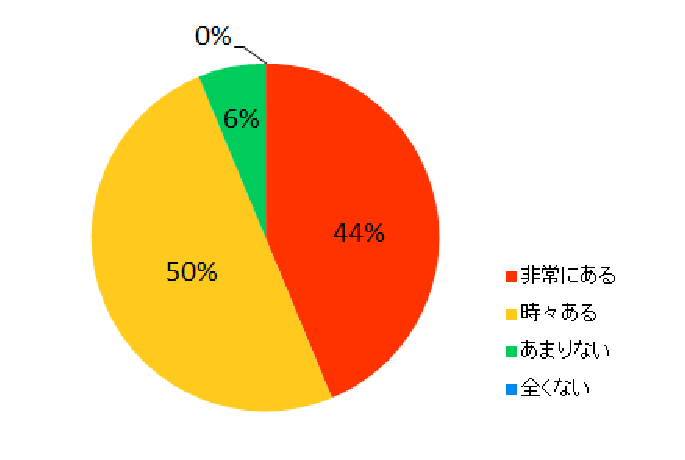
\includegraphics[width=6cm]{fig/chap1/Q1-1.eps}}
	\subcaptionbox{\textgt{吹奏楽・オーケストラ未経験者の回答}
		\label{fig:ans1_2}}{
		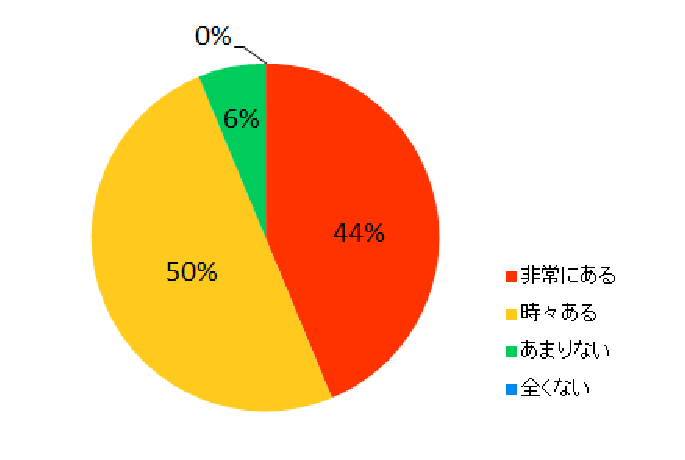
\includegraphics[width=6cm]{fig/chap1/Q1-2.eps}}
	\caption{演奏アニメーションが不自然であると感じることがあるかどうか}
	\label{fig:q1}
\end{figure}

これらの違和感や不自然さを解消するためには,身体の動きを1つずつ音階やリズムなどに,手動で合わせる必要がある.
この方法はひじょうに効率が悪く,多くの時間と労力が必要となる.

\section{研究目的}\label{sec:purpose}
\indent
\secref{sec:background}節で述べた課題を解消するため,本研究では,管楽器を演奏するキャラクタの吹奏アニメーションを,音源から自動的に生成することを目指す.
より具体的には,実際の演奏アニメーション制作フローに沿わせるため,楽曲は電子楽器を用いて,MIDI(Musical Instrument Digital Interface)音源として生成する.
次に,作成した楽曲を解析することにより,吹奏の情報を得る.
最後に,得られた情報をキャラクタの身体の動きや表情,そして管楽器に適用することにより,音源に同期した自然な吹奏アニメーションを実現する.
提案手法の対象ユーザはアニメータとし,最終的にはアニメータのアニメーション制作時間と労力の削減を目的とする.
また,本研究は,同研究室学士4年の武内と共同で行った.
武内が担当した部分については,その旨を明記する.

\section{本論文の構成}\label{sec:structure}
本論文は次章以降,以下のように構成される.\\
\indent
次章では関連研究を説明する.
第3章では提案手法の仕組みを説明する.
そして,第4章では自動生成結果を述べ,この結果に対する評価をまとめる.
最後に第5章で結論を述べ,今後の課題に言及する.\\
\indent
なお,本研究の成果はVisual Computing/グラフィクスとCAD合同シンポジウム2017にてポスター発表\cite{vc}を行った.そして,映像表現・芸術科学フォーラム2018(2018年3月),Cyberworlds(2018年8月)において発表を行う予定である.
%%%% 従来の研究
\chapter{関連研究}
\label{chap:previousworks}
本章では関連研究に言及する.
まず,\secref{sec:generate_animation}で音からアニメーションを自動生成する研究を紹介し,\secref{sec:generate_sound}でアニメーションから音を自動生成する研究を紹介する.
\secref{sec:synchronization}で音とアニメーションを同期させる研究,
\secref{sec:animoji}でユーザの表情をキャラクタに反映させる研究,
\secref{sec:marching}で吹奏楽に関連した研究を紹介する.
最後に\secref{sec:compere}にて本研究の新規性を述べる.

\section{音からアニメーションを自動生成する研究}\label{sec:generate_animation}
音とアニメーションを同期させることを目的として,音からアニメーションを自動生成する研究は多く存在している.\\
\indent
物が落下するアニメーションを生成するには,物の落下音と物が落下するタイミングを1つずつ合わせる必要がある.
Langloisら\cite{IFA}は,それらを正確に合わせるために,物が落下する音が収録されている音源から,物が落下するアニメーションを自動生成する手法を提案した.\\
%\begin{figure}[h]
%	\centering
%	
\includegraphics[width=15cm]{fig/chap2/IFA.eps}
%	\caption{落下アニメーションの自動生成結果}
%	\label{fig:IFA}
%\end{figure}
%
\indent
キャラクタの口の動きと音声を同期させる,リップシンクという技術がある.
キャラクタの口の動きに合わせて後から音声を録音するアフレコは,アニメーションに合わせて台詞を収録するため,口元と台詞の同期が比較的容易である.
一方,音声に合った口元のアニメーションを生成するには,口の形や動きを音声と1つずつ合わせる必要がある.
また,映画の吹替え版では,役者の口と声にズレが生じることに,違和感を感じることがある.
上述の課題を解消するため,リップシンクは,近年注目を集めている技術の1つである.\\
\indent
Breglerら\cite{Bregler},Ezzatら\cite{Ezzat}は,既存の動画に映っている対象人物の口元のみを,音声データに合わせて再構成することにより,リップシンクを図る手法を提案した.
Edwardsら\cite{JALI}は,台詞が収録されている音源および台詞が記載されているテキストファイルを入力すると,その台詞を話している口元のアニメーションを自動生成する手法を提案した.
本手法では,顎と唇だけを制御することにより,自然な口元のアニメーションを自動生成している.さらに,後から表情を編集することが可能となっているため,より自然な表情のアニメーションを実現できる.\\
%\begin{figure}[h]
%	\centering
%	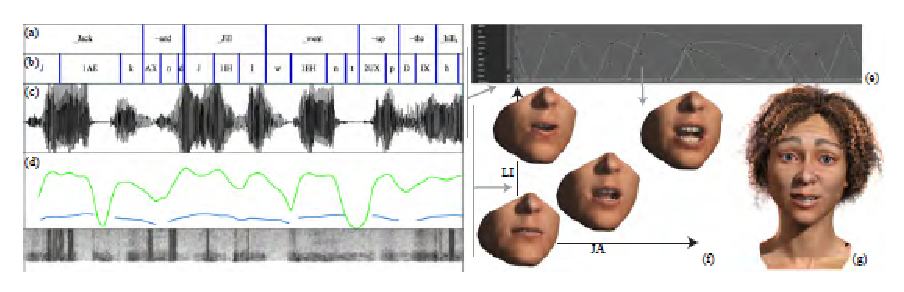
\includegraphics[width=15cm]{fig/chap2/JALI.eps}
%	\caption{口元アニメーションの自動生成}
%	\label{fig:JALI}
%\end{figure}
%
\indent
本研究の目的と同じように,音源から楽器を演奏するアニメーションを自動生成する研究も行われている.
Zhuら\cite{piano}は,MIDI音源からピアノを弾く指元のアニメーションを自動生成する手法を提案した.
ピアノのような鍵盤楽器は,指と音が一対一で対応していないため,フレーズにより指使いを変える必要がある.
ある指が他の指の上や下を通るような指使いのときは,指同士が衝突しないように考慮する必要もある.
彼らの手法では,これらの課題を解消することが可能である.\\
\indent
Yinら\cite{violin}は,wave音源からバイオリンを弾く手のアニメーションを自動生成する手法を提案した.
彼らは弦を押さえる左手の指元のアニメーションだけでなく,その指の動きが不自然に見えないような手首や腕の動きも再現している.
加えて,弓を持つ右手の動きも自動生成している.
Kimら\cite{violin2}も同様に,バイオリンを引く手のアニメーションを自動生成する手法を提案した.\\
\indent
ElKouraら\cite{ElKoura}は,ギターを弾く左手のアニメーションを自動生成する手法を提案した.
彼らの研究はギターの弾き方の指導を目的としており,アニメーションは音源から自動生成するのではなく,指を置く位置を入力することで生成される.\\
%\begin{figure}[h]
%	\centering
%	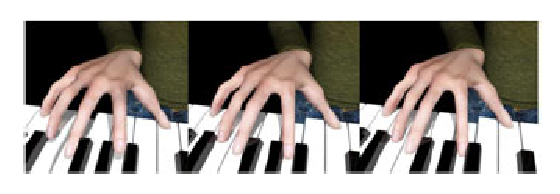
\includegraphics[width=15cm]{fig/chap2/piano.eps}
%	\caption{ピアノを弾く手元のアニメーションの自動生成}
%	\label{fig:piano}
%\end{figure}
%
\indent
上述の研究の他にも,音源に合った表情を自動生成する研究\cite{facial}\cite{DiPaola}\cite{morishima}や,音源に合ったダンスアニメーションを自動生成する研究\cite{dance2}\cite{dance1}など,さまざまなジャンルに着目した研究が存在する.

\section{アニメーションから音を生成する研究}\label{sec:generate_sound}
音とアニメーションを同期させることを目的として,物理シミュレーションの結果を音に反映させる研究分野が存在する.
以下では,その分野に関連した研究を紹介する.\\
%
\subsection{サウンドレンダリング}
サウンドレンダリングとは,物理アニメーションを生成すると同時に音を生成することにより,双方を同期させることを目的とする研究分野である.
この分野は,1992年に発表されたTakalaらの論文\cite{sound}が発端となっている.
彼らは,音の実態が光と同じ波動であること,音が物体の動きに依存することに着目して,音をレンダリングにより自動生成する手法を提案した.
%CG-ARTSの教育リポート,『音を描き出す夢の実現』\cite{CG-ARTS}によると,本分野は1990年代前半に登場し,未だ実験的にとどまっている分野となっている.
2009年には1つのシミュレーションパイプラインのなかで,CGアニメーションと,それに呼応した音を同時に生成するアルゴリズム\cite{james1}がZhengにより考案された.
本アルゴリズムでは,自然な流水音が,流水アニメーションから自動生成される.
また,自動生成された流水音は,アニメーションと完全に同期している.
%\begin{figure}[h]
%	\centering
%	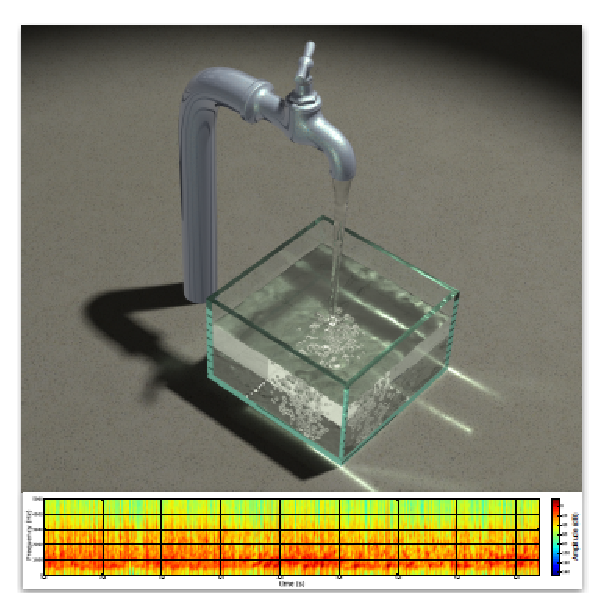
\includegraphics[width=15cm]{fig/chap2/james1.eps}
%	\caption{水のアニメーションと音の同時生成結果}
%	\label{fig:james1}
%\end{figure}
%
翌年には,同氏らにより破壊音を自動生成するアルゴリズム\cite{james2}が発表された.
本アルゴリズムでは,さまざまな剛体の破壊音だけでなく,その衝撃が間接的におよぼす影響も考慮されている.
そのため,複数の物体がぶつかり合い,破壊し合うようなアニメーションでも,そのアニメーションに同期する音が,忠実に再現された.
%\begin{figure}[h]
%	\centering
%	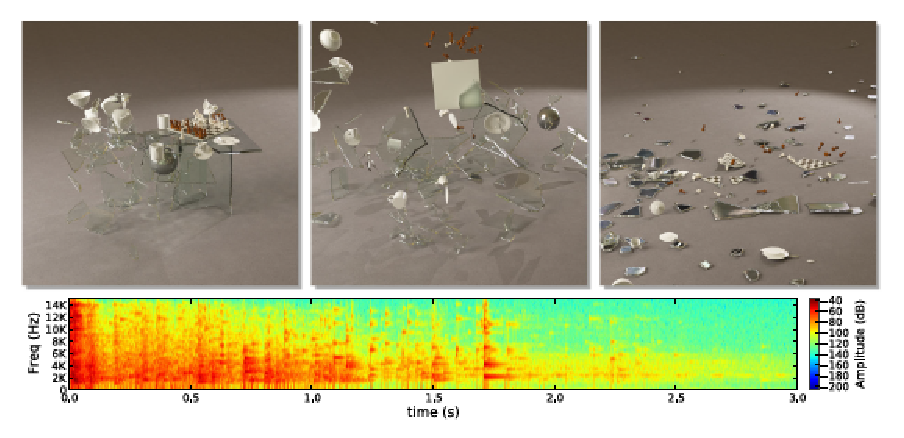
\includegraphics[width=14cm]{fig/chap2/james2.eps}
%	\caption{複数の剛体がぶつかり破壊される様子}
%	\label{fig:james2}
%\end{figure}
%
\subsection{プロシージャルオーディオ}
プロシージャルオーディオとは,作り置きした音を必要なタイミングで再生するのではなく,その都度プログラムで作り出す技術である.
ゲームソフトを開発している株式会社スクウェア・エニックスは本技術を研究しており,2014年のCEDECにて詳細\cite{SQUARE}を発表した.\\
\indent
ゲームでは,プレイヤの操作に応じてシステム内で効果音が選択され,再生される.
それらの音は,一般的には事前に作成し,システムに記憶させておく.
しかし,ゲームは使用可能な記憶領域が限られているため,可能な限りメモリを節約したい.
そのようなときに,本技術はひじょうに役立つ.
また,物体の挙動に合わせて音を自動生成するため,自然な効果音を再現することができる.

\section{音とアニメーションを同期させる研究} \label{sec:synchronization}
音やアニメーションを,もう一方から自動生成する研究だけでなく,既に生成されている双方を編集することにより同期させる研究も存在する.
Leeら\cite{Lee}は,MIDI音源およびキャラクタのモーションデータを入力とし,双方を最小限編集することにより,MIDI音源と同期したキャラクタのダンスアニメーションを生成する手法を提案した.\\
%\begin{figure}[h]
%	\centering
%	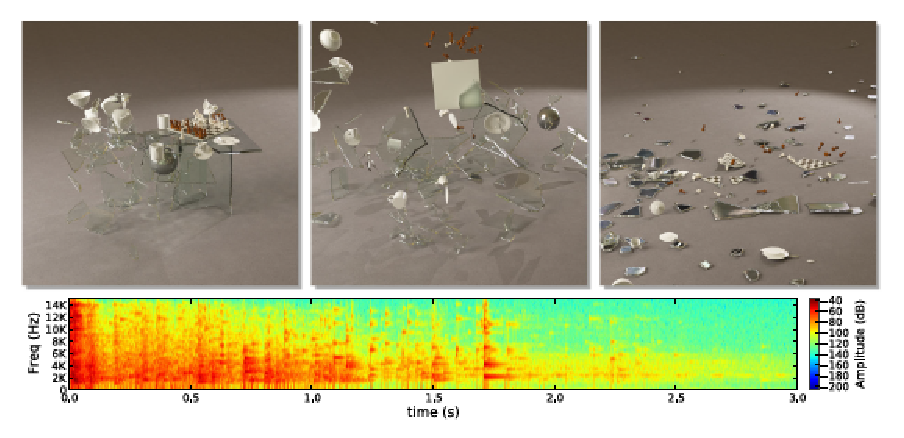
\includegraphics[width=15cm]{fig/chap2/james2.eps}
%	\caption{ダンスアニメーションと音を同期}
%	\label{fig:lee}
%\end{figure}
\indent
この研究分野は,複数のカットを組み合わせて作成するモンタージュの作成にも応用されている.
Liaoら\cite{Liao}は,BGMとなる音源および複数のビデオクリップを入力することにより,BGMに合ったモンタージュを作成する手法を提案した.

\section{ユーザの表情をキャラクタに反映する研究} \label{sec:animoji}
2017年秋に発売されたiPhoneXには,アニ文字という機能がある.
この機能は,カメラで認識したユーザの表情を,デバイス内のキャラクタに反映することができる.
このように,ユーザの表情をカメラで認識することにより,キャラクタのフェイシャルアニメーションを自動生成することを目的とした研究が存在する.\\
\indent
Weiseら\cite{Weise}は,カメラを用いてユーザの顔のモーションをキャプチャすることにより,顔のモーションデータを取得し,
それを仮想世界のキャラクタの顔に反映する手法を提案した.
顔のモーションキャプチャにはマーカーが必要がない.
また,キャプチャ中に手などにより顔が遮られた場合は,自動的に補正される仕組みとなっている.
なお,反映されるキャラクタは,人型のキャラクタのみである.
この研究を行っていたメンバーの1人であるPauly\cite{Pauly}は,2年後に,トラッキングの際に深さを考慮することにより,トラッキングの質を向上させた.
そのことにより,しわなど皮膚の細かい情報もキャラクタに反映されるようになった.\\
\indent
同年にXuら\cite{Xu}は,顔のモーションデータを人型ではないキャラクタの顔に反映する手法を提案した.

\section{吹奏楽に関連した研究} \label{sec:marching}
マーチングとは,演奏者が演奏しながら定められた経路に従って歩くことにより隊形を作る,吹奏楽の演奏形態である.
本論文の筆者は,マーチングを行う1名の演奏者の軌跡を可視化することにより,その演奏者が歩くべき経路と実際の経路の誤差を表示するシステム(\figref{fig:marching})を提案した.
軌跡の可視化には,物体追跡アルゴリズムの1つであるLucas Kanade法\cite{Lucas}が用いられている.
本システムにより,演奏者は自身の歩行の改善点を知ることができ,その結果マーチングの隊形の完成度を高めることが期待できる.
\begin{figure}[H]
	\centering
	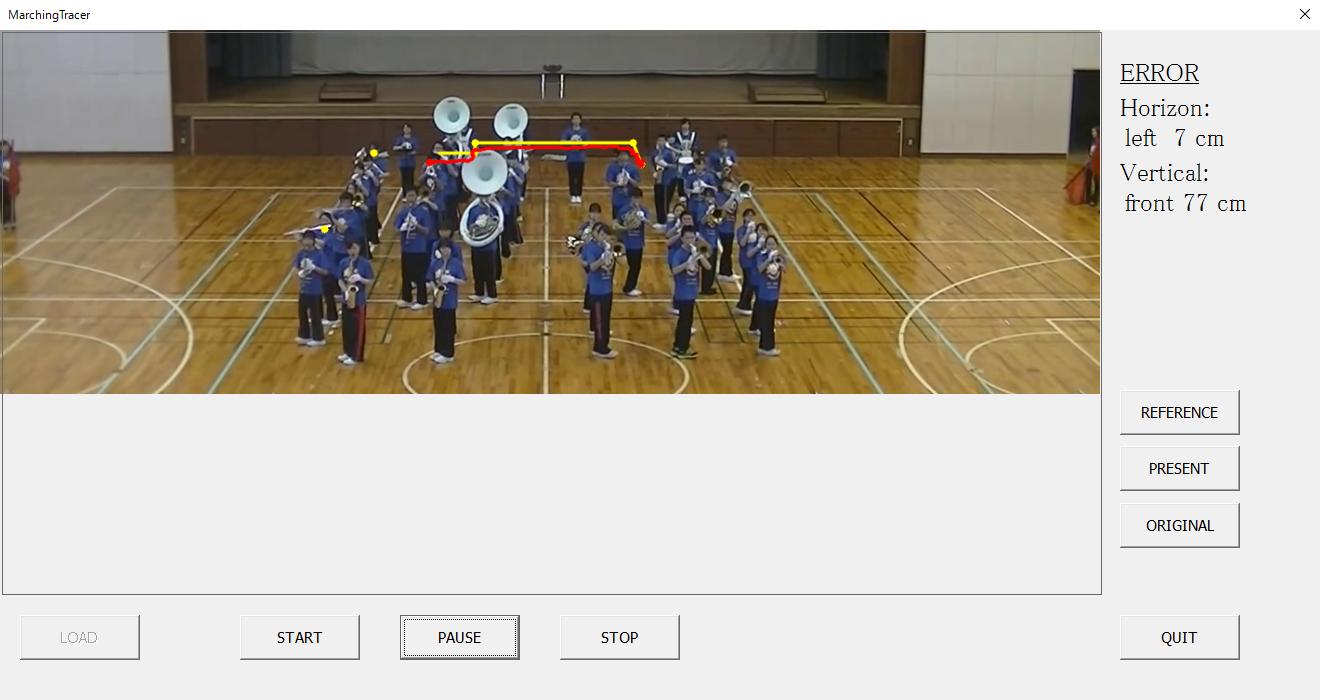
\includegraphics[width=14cm]{fig/chap2/marching.eps}
	\caption{マーチングを行う演奏者の軌跡および誤差の表示例}
	\label{fig:marching}
\end{figure}
なお,この研究の成果は,NICOGRAPH2016においてポスター\cite{nicograph}にて発表した.
そして,一連の研究をまとめた成果が,画像電子学会誌のVol.47\cite{iieej}に掲載される予定である.

\section{本研究の新規性}\label{sec:compere}
アニメーションと音の同期や,吹奏楽をテーマとした研究は多く存在する.
しかし,管楽器を演奏するキャラクタと音の同期に注目した研究は存在しない.
また,\secref{sec:generate_animation}で挙げた,ピアノやバイオリンを演奏するアニメーションの自動生成を目的とした研究では,複数名での演奏は考慮されていない.
したがって本研究の新規性は,管楽器を複数名で演奏するアニメーションを,音から自動生成するという点である.
さらに,本論文ではトランペット奏者およびトロンボーン奏者に適用した例だけを示すが,音と指使いの対応表を用意することにより,すべての管楽器の演奏アニメーションが入力音源から自動生成できる.
このように,あらゆる楽器への対応が可能である点も,新規性があるといえる.
%%%% 本研究のアプローチ
\chapter{提案手法} \label{chap:algorithm}
本章では提案手法を詳しく説明する.
まず,\secref{flow}にて自動生成の大まかな流れを説明し,その後にそれぞれの工程について詳しく述べる.
\secref{input}および\secref{output}にて入出力について説明し,
\secref{device}にて使用するデバイス,
\secref{software}にて使用するソフトウェア,
\secref{3Dmodel}にて使用する3Dモデルについて述べる.
\secref{analysis}にてMIDIデータの解析からモーションへの適用方法を説明する.
そして最後に,\secref{howto}にて実際にシステムを使用する際の,使用方法について言及する.

\section{自動生成の流れ} \label{sec:flow}
\figref{fig:flow}に,音源から吹奏アニメーションを自動生成する流れを示す.\\
\begin{figure}[h]
	\centering
	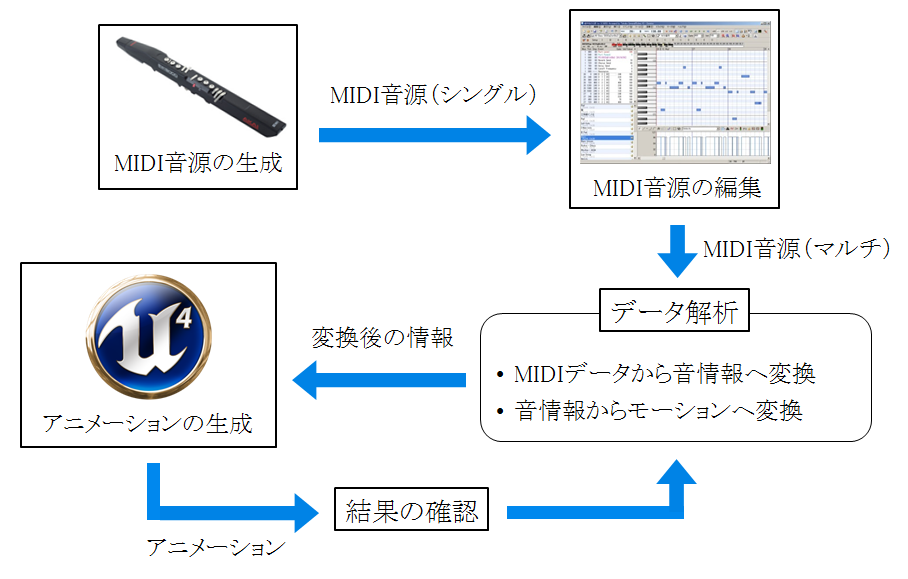
\includegraphics[width=14cm]{fig/chap3/flow.eps}
	\caption{音源から吹奏アニメーションを自動生成する流れ}
	\label{fig:flow}
\end{figure}
\indent
実際のアニメーション制作フローに沿わせるため,音源の生成は楽器を用いて行う.
次に,生成した音源を解析し,譜面データへ変換する.
そして,アニメーション生成と同時に音源を流すことにより,音源に合わせてキャラクタが動くアニメーションが完成となる.

\section{入力} \label{sec:input}
入力する音源は,MIDI音源とする.
ここで,MIDI音源は,MIDIという信号を受信して発音する音源のことである.
よく使用されるmp3やwaveなどの形式とは異なり,中身が譜面データとなっているため,音の解析が比較的容易である.\\
\indent
このMIDI音源を生成する方法は,後述する.

\section{出力} \label{sec:output}
出力は,管楽器を演奏するキャラクタのアニメーションである.
今回対象とする管楽器は,トランペット,トロンボーンである.
この2本の楽器を選んだ理由は,吹奏楽ではとくに目立つ楽器であり,3Dモデルが入手しやすかったために選んだ.

\section{デバイス} \label{sec:device}
MIDI音源を生成するために,電子楽器であるウインドシンセサイザ「EWI5000」(\figref{fig:ewi})を使用する.
このウインドシンセサイザは,さまざまな楽器の音を再現することが可能である.
\begin{figure}[h]
	\centering
	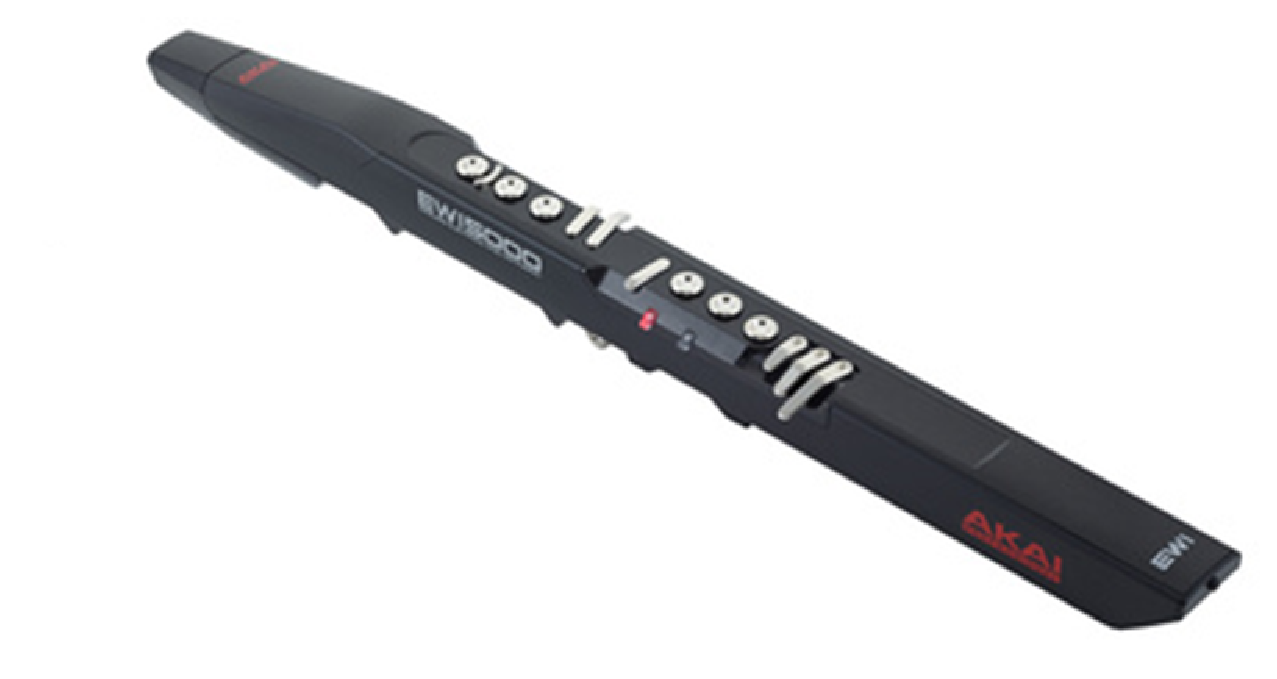
\includegraphics[width=10cm]{fig/chap3/ewi.eps}
	\caption{ウインドシンセサイザ「EWI5000」}
	\label{fig:ewi}
\end{figure}

\section{ソフトウェア} \label{sec:software}
\secref{device}で述べたウインドシンセサイザは,単音しか鳴らすことができないため,シングルチャンネルの音源しか生成することができない.
しかし,吹奏アニメーションを自動生成するためには,複数人で演奏しているマルチチャンネルの音源が必要となる.
そこで,ウインドシンセサイザで生成したMIDI音源を,フリーソフトウェアであるMIDIシーケンスソフトウェア「Domino」(\figref{domino})に出力し,重ねて何度も録音することにより,マルチチャンネルの音源を生成する.
\begin{figure}[h]
	\centering
	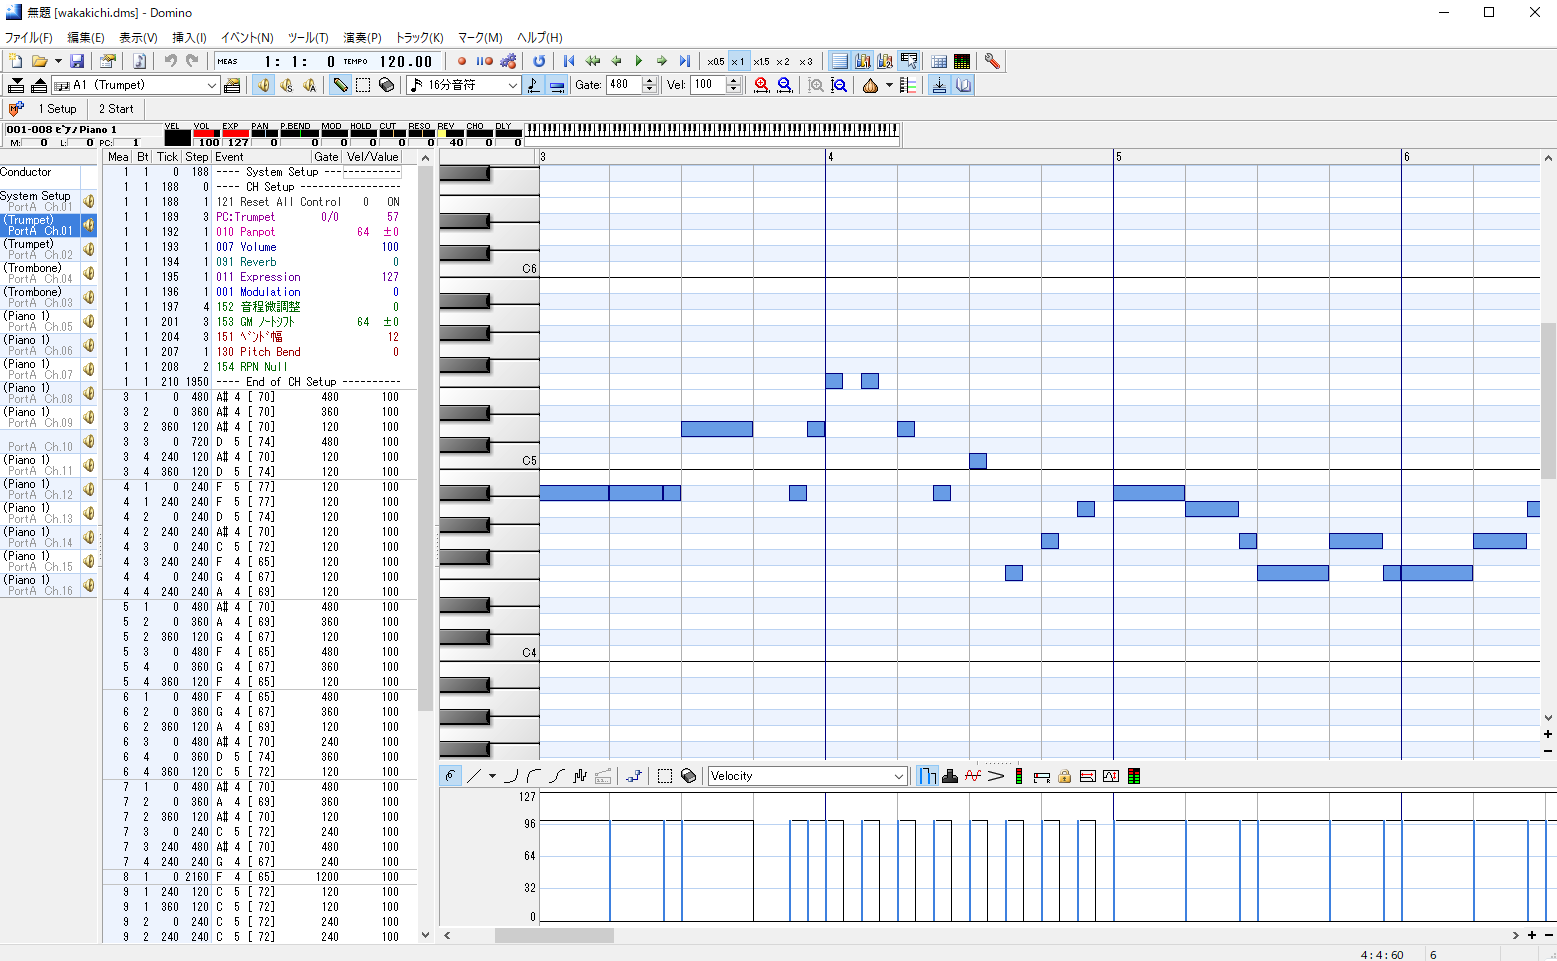
\includegraphics[width=10cm]{fig/chap3/domino.eps}
	\caption{MIDIシーケンスソフトウェア「domino」}
	\label{fig:domino}
	
\end{figure}

\section{3Dモデル} \label{sec:3Dmodel}

\section{MIDIデータの解析} \label{sec:analysis}

\subsection{楽譜データへの変換}

\subsection{モーションへの適用}

\section{本システムの使用方法} \label{sec:howto}
%%%% アルゴリズム
\chapter{結果と評価}
\label{chap:results}
本章では,3章で紹介した手法によって自動生成した吹奏アニメーションについて記述する.
\secref{sec:system}では仕様したPCやシステムの仕様を述べ,
\secref{sec:result}では自動生成した吹奏アニメーションのキャプチャリング画像を示す.
そして\secref{sec:review}では自動生成結果を実際の演奏シーンや既存の吹奏アニメーションと比較することにより,提案手法を評価する.

\section{実行環境} \label{sec:system}
事前にUnreal Engineにて専用のプロジェクトを作成し,モーションのデータが記載されているUnreal Engine専用のファイルをインポートする.
そして,キャラクタと,それぞれが演奏する楽器を\figref{fig:ue4}のようにセッティングする.
なお,最初にインポートするUnreal Engine専用のファイルには,キャラクタの姿勢データも存在するため,
キャラクタの姿勢のセッティングは容易にできる.\\
\indent
実行環境は\tabref{tab:pc}の通りである.
\begin{figure}[h]
	\centering
	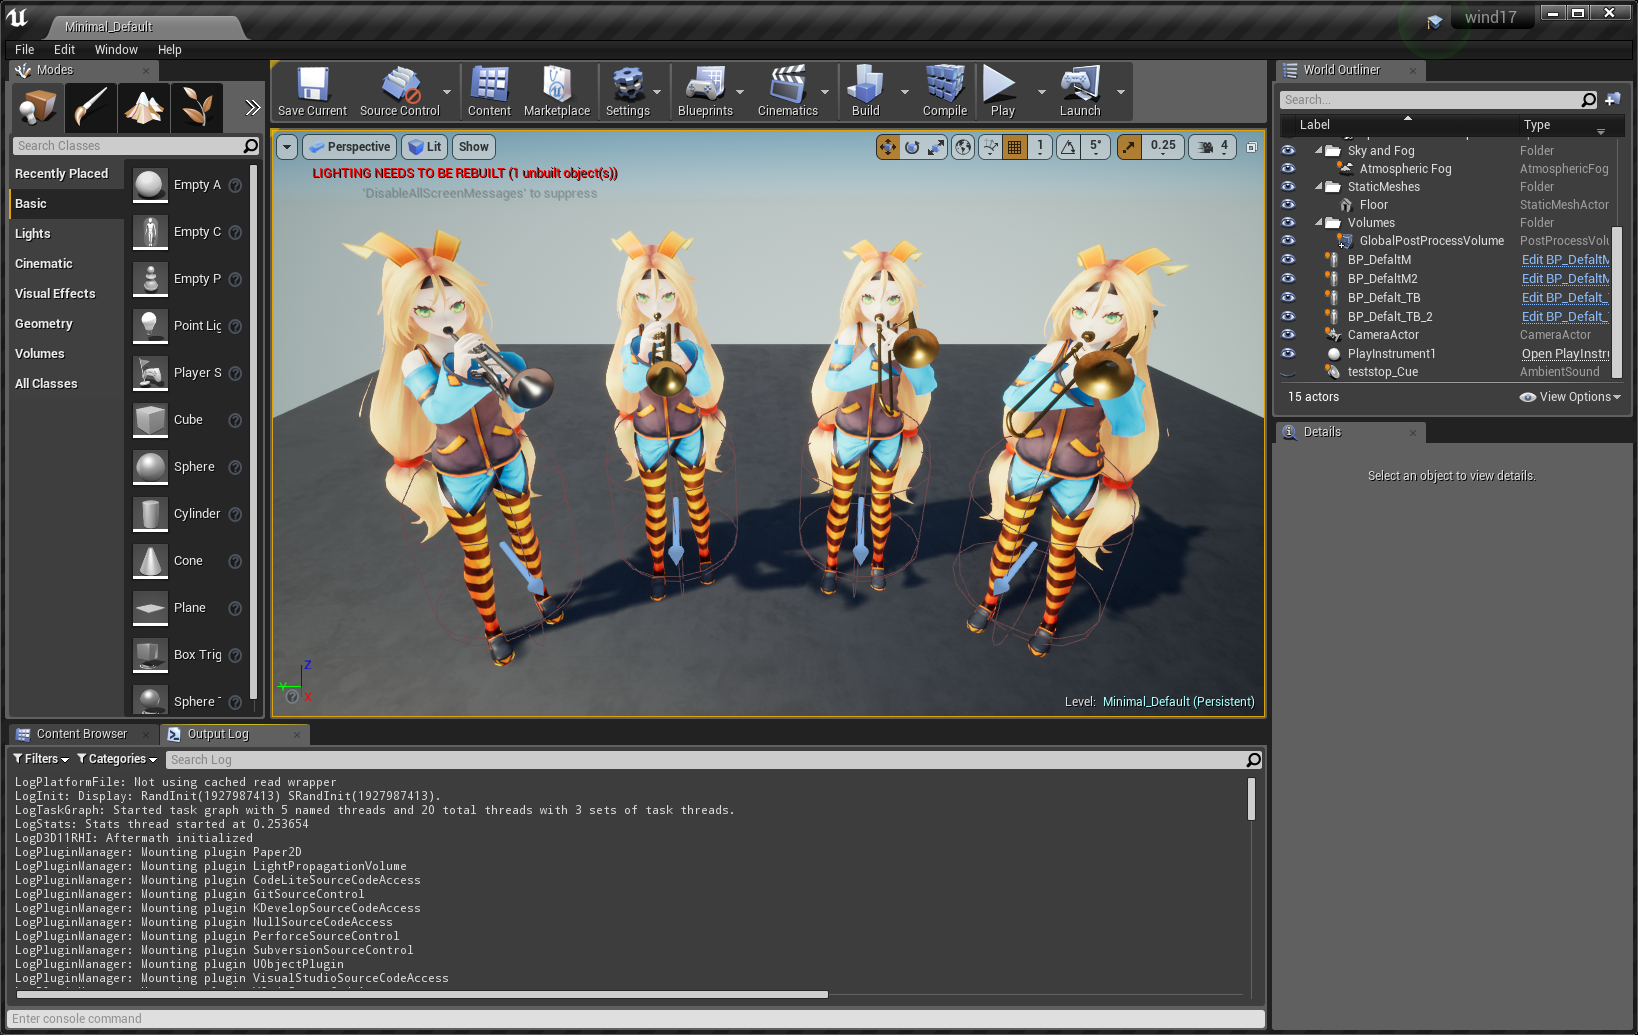
\includegraphics[width=14cm]{fig/chap4/ue4.eps}
	\caption{Unreal Engineの初期設定}
	\label{fig:ue4}
\end{figure}

\begin{table}[htbp] 
	\begin{center}
		\caption{実行環境}
		\label{tab:pc}
		\begin{tabular}{|l|c|}
			\hline
			OS & Windows10 64bit \\ \hline
			CPU & Intel\textregistered Core\textsuperscript{TM}i7-3930K \\ \hline
			RAM & 32.00GB\\ \hline
			言語 & c++\\ \hline
		\end{tabular}
	\end{center}
\end{table}

\section{アニメーション生成結果} \label{sec:result}
本研究で作成したアニメーションは,主に少人数編成であるアンサンブルアニメーションである.
以下では,トランペット奏者2名で演奏するアニメーションのキャプチャリング画像と,
トランペット奏者2名,トロンボーン奏者2名の計4名で演奏するアニメーションのキャプチャリング画像を示す.
以下,それぞれについて制御している口元やボーンの制御について説明するが,
前者のアニメーションは口元や指元がズームインされているシーンであるため,主に口元や指元のボーンの制御について,
後者のアニメーションは全体を俯瞰しているシーンであるため,主に指元以外のボーンの制御について述べる.\\
\indent
\figref{anim1}は,トランペット奏者2名の基本姿勢である.
\begin{figure}[h]
	\centering
	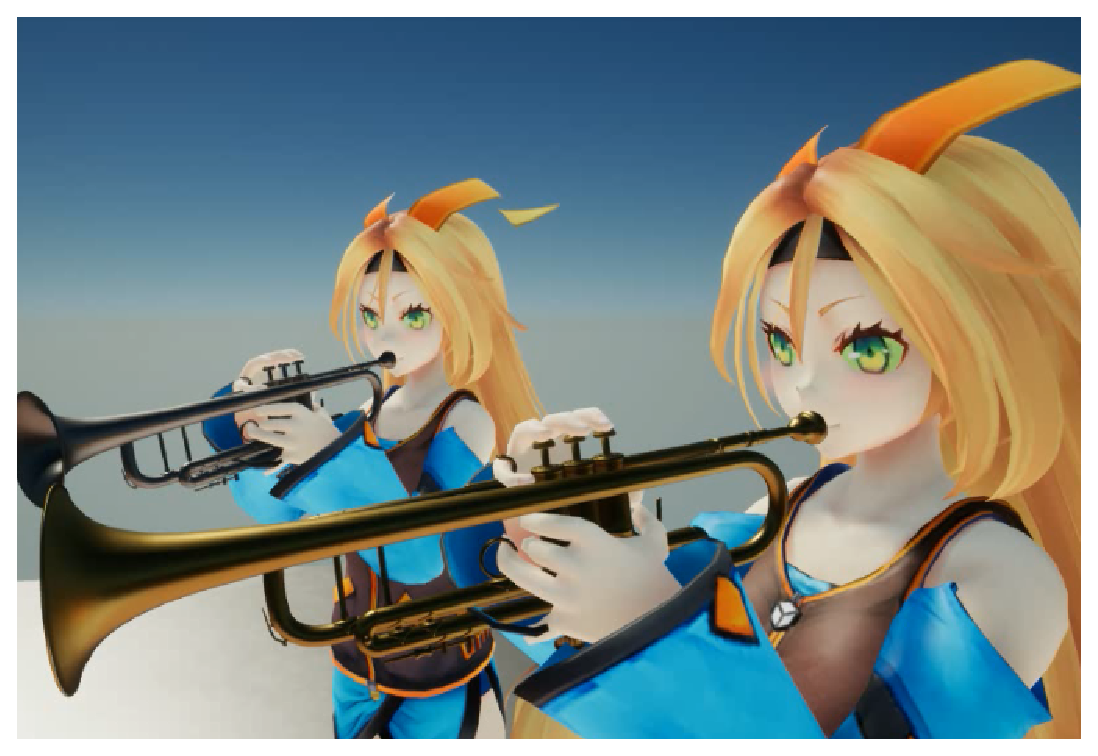
\includegraphics[width=10cm]{fig/chap4/anim1.eps}
	\caption{トランペット奏者2名の基本姿勢}
	\label{fig:anim1}
\end{figure}
音を鳴らすタイミングで,演奏者は\figref{anim1_finger}のように,指でトランペットのピストンを押す動作をする.
\begin{figure}[h]
	\centering
	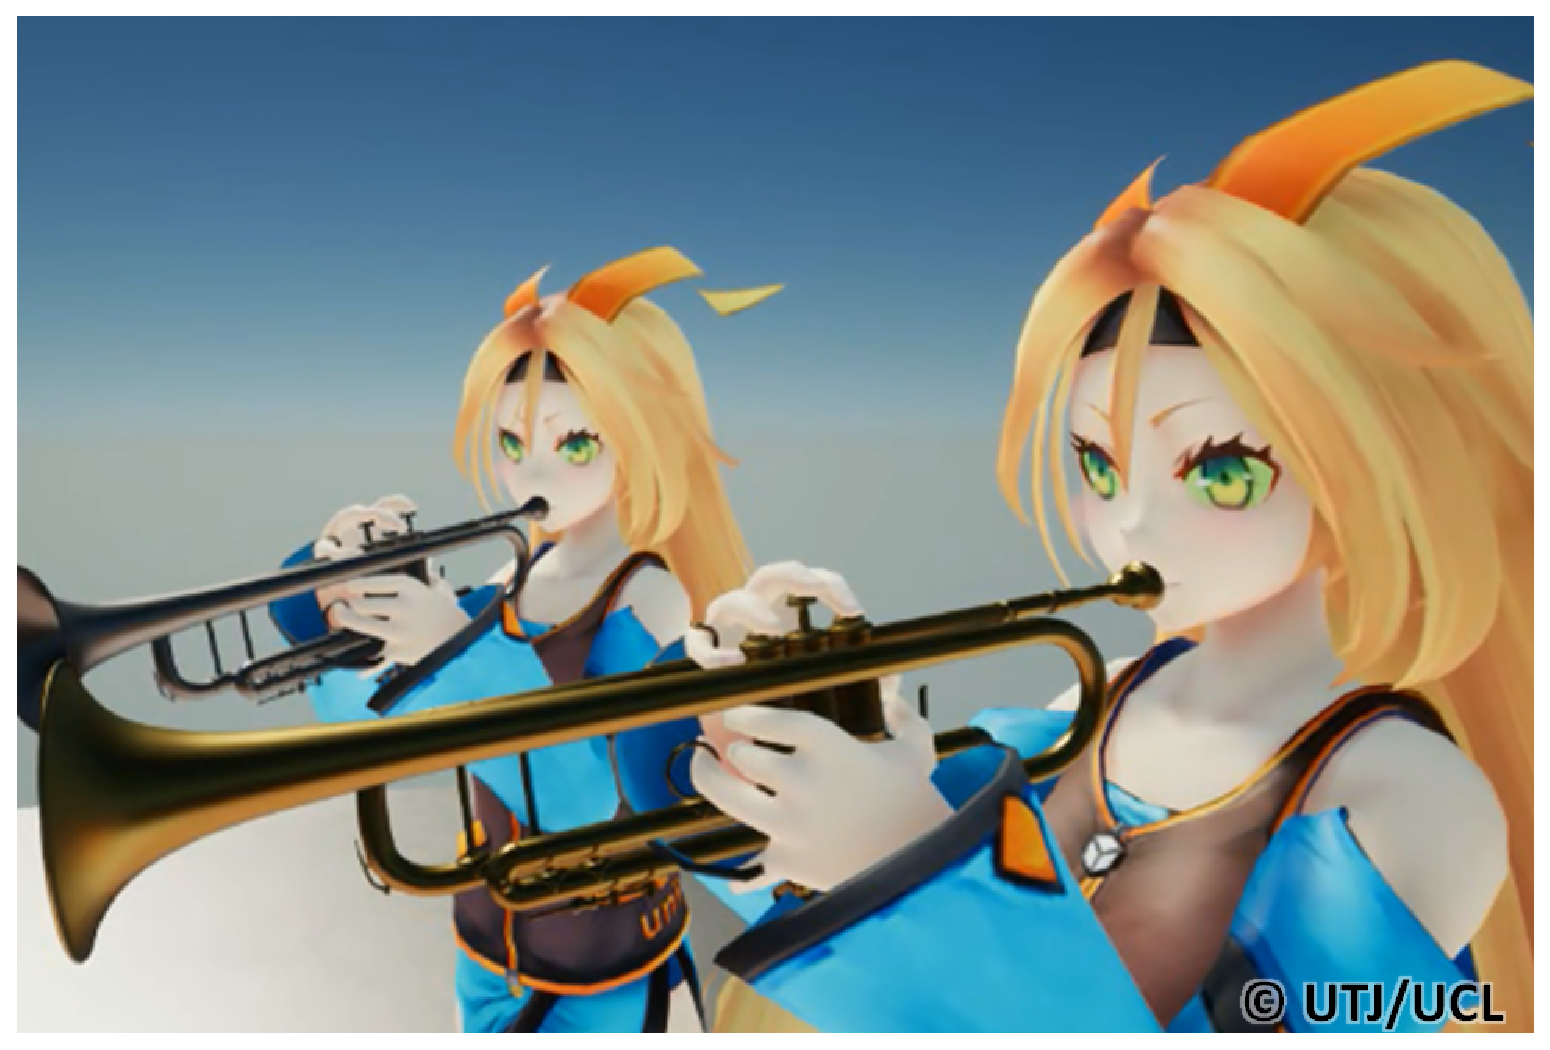
\includegraphics[width=10cm]{fig/chap4/anim1_finger.eps}
	\caption{トランペット奏者2名がピストンを押す姿勢}
	\label{fig:anim1_finger}
\end{figure}


\section{評価} \label{sec:review}

\subsection{実際の演奏シーンとの比較による評価}

\begin{figure}[t]
	\centering
	\subcaptionbox{\textgt{吹奏楽・オーケストラ経験者の回答}
		\label{fig:unity}}[0.75\linewidth]{
		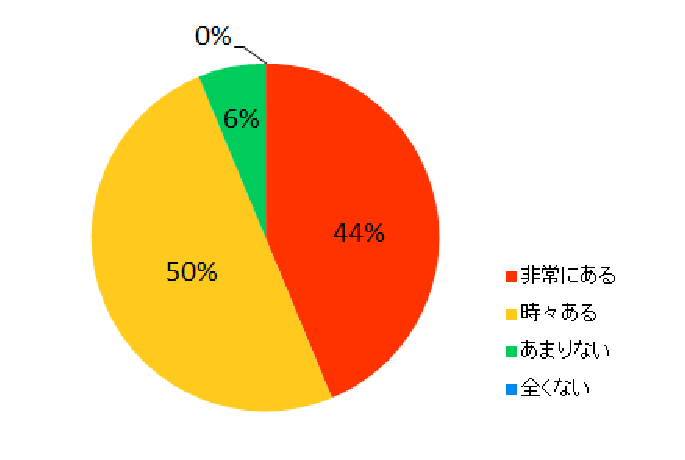
\includegraphics[height=7cm]{fig/chap1/Q1-1.eps}}
	\subcaptionbox{\textgt{吹奏楽・オーケストラ未経験者の回答}
		\label{fig:tp}}[0.6\linewidth]{
		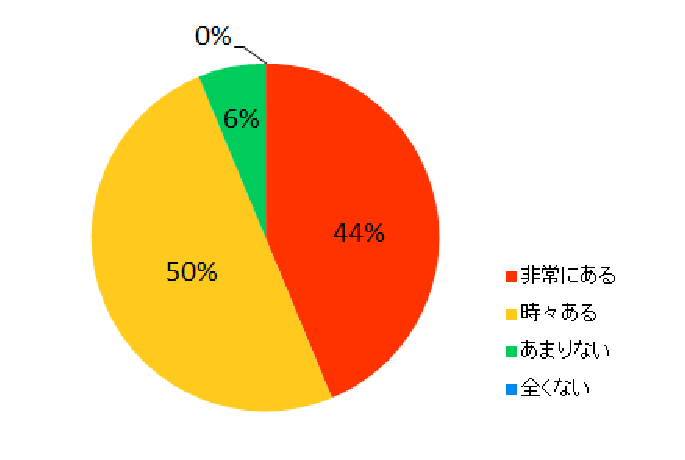
\includegraphics[height=5.5cm]{fig/chap1/Q1-2.eps}}
	\caption{演奏アニメーションが不自然であると感じることがあるかどうか}
	\label{fig:model}
\end{figure}

\subsection{既存のアニメーションとの比較による評価}

\subsection{アンサンブルアニメーションの評価}

\subsection{システムの有用性の予想}
%%%% 結果と評価
\chapter{結論}
\label{chap:conclusion}
本章では本論文の結論を述べ,今後の課題に言及する.

\section{まとめ}
本論文では,音源から演奏アニメーションを自動生成することにより,音源に同期したアニメーションを自動生成する手法を提案した.
音情報を容易に解析できるMIDI音源を使用し,そこから得た演奏の情報をUnreal Engine のキャラクタに適用することにより,運指や表情が音源に同期した吹奏アニメーションを,短い時間,少ない労力で生成することができた.
特に音と1対1で対応するトランペット奏者の指元やトロンボーン奏者の腕の動きは,音と完全に同期した動きを再現できた.
複数名で演奏するアンサンブルアニメーションでは,それぞれの動きのパラメタを0から1で割り当てることにより,基となる1つのモーションを,見た目が異なるモーションとして演奏者全員に適用できた.

\section{今後の課題}
今後の課題として挙げられるのは,表情やモーションの種類の向上,モーションと音の関連付け,楽器や演奏者の増加である.
本節では,それぞれについて詳しく説明する.

\subsection{表情の豊かさの向上}
{\gt3.8.2項}で口元の制御について述べたが,演奏する際に変化する表情は口元だけではない.
他の演奏者と目配せをすることや,音が長くて息継ぎできない場合,音が高い場合に辛そうな表情をすることがある.
楽器に息を入れる際に頬が膨らむ演奏者もいる.
これらの表情の変化もモデルに適用することにより,表情の豊かさが向上し,より自然なアニメーションが完成すると考えられる.
方法としては,音の長さなどから判断できる情報については,音情報から自動的に算出,感情の変化のような,音情報から判断しづらい情報については,表情の遷移を記載するメタデータを用意することが挙げられる.\\
\indent
しかし,目配せや辛い表情など,あらゆる表情の再現は,現状ではUnreal Engineのみでは不可能である.
口元を制御する際,Unreal Engineのモーフターゲットという機能を用いているが,この機能はブレンドシェイプが適用されていないメッシュには使用できない.
ここで,ブレンドシェイプとは,あらかじめ用意された複数の表情モデルをパラメタの調整により組み合わせることで,さまざまな表情を作成するアニメーション手法をさす.
今回用いたユニティちゃんは,デフォルトで口元にブレンドシェイプが設定されているため,モーフターゲットによる口元の制御は可能であるが,
目配せや辛い表情などを再現するためのブレンドシェイプは,デフォルトの設定では不足している.
そのため,あらゆる表情を再現するためには,他のソフトウェアを介してブレンドシェイプを設定する必要がある.

\newpage
\subsection{モーションの種類の向上}
自動生成したアニメーションと実際の演奏シーンと比較すると,キャラクタの動きに不自然な点が見つかる.
その原因の1つとして,モーションの種類が少ないことが挙げられる.
楽器を演奏する際の身体のモーションについては{\gt3.8.3項}で触れたが,ここで述べたモーションだけでは足りない.
例えば,音の高低に合わせて楽器を上下に揺らす演奏者や,円を描くように楽器を揺らす演奏者がいる.
これらのモーションを追加し,モーションの種類を増やすことにより,さまざまな表現の実現が可能になり,より自然な吹奏アニメーションの自動生成が可能になると考えられる.

\subsection{モーションと音の関連付け}
自動生成したアニメーションと実際の演奏シーンを比較したときに,キャラクタの動きが不自然に見える原因として他に考えられるのが,モーションと音の関連付けが完璧でない点である.
現在は,曲のテンポに従って身体が動く仕組みとなっており,モーションの種類や大きさは,ランダムに選択される仕様となっている.
より自然な吹奏アニメーションを自動生成するためには,音の遷移とモーションを1対1で対応させたり,モーションを事前に指定するためのメタデータを用意することにより,モーションと音を関連付ける必要がある.

\subsection{楽器の種類および演奏者の増加}
本論文では吹奏楽の1つの演奏形態であるアンサンブルを想定し,楽器はトランペットとトロンボーンを選択したが,アンサンブルで使用される楽器はこの2本だけではない.
また,将来的には大人数で曲を合奏している吹奏アニメーションの再現を目指す.
そのため,楽器のモデルを増やす必要がある.
{\gt3.8.1項}の\tabref{tab:map}に示したような音と運指の対応表を作成することにより,トランペット,トロンボーンと同じように吹奏アニメーションの再現が可能となる.
また,今回は演奏者としてユニティちゃんを選択しているため,全員同じ体型であるが,実際演奏者それぞれの体型は異なっている.
体型に関わらず自然な吹奏アニメーションを生成するには,リターゲティングのための追加実装や,動きの差を記述するメタデータが必要となる.
%%%% 謝辞
\chapter*{�ӎ�}
\label{chap:thanks}



\renewcommand{\refname}{公開文献}	
%
\begin{thebibliography}{55}
\addcontentsline{toc}{chapter}{公開文献}% 追加
%
\bibitem[i]{nicograph}
堀井 絵里,藤代 一成,
``マーチングバンドにおける演奏者個人を対象とした移動経路の計量可視化",芸術科学会 NICOGRAPH2016 予稿集,pp.119-120,2016年11月.

\bibitem[ii]{iieej}
堀井 絵里,藤代 一成,``マーチングバンドの演奏者個人に注目した移動経路の計量可視化",画像電子学会誌,Vol.\,47,No.\,1,2018年1月(掲載予定).

\bibitem[iii]{vc}
堀井 絵里,藤代 一成,``音源に同期する運指に注目した吹奏アニメーションの自動生成",Visual Computing/グラフィクスとCAD合同シンポジウム 2017 DVD 予稿集,No.\,41,2017年6月.

%\bibitem[iv]{vc}
%池田 泰成,松岡 徹,藤代 一成,「頭髪状物体の影のオブジェクトスペースアンチエイリアシング」,電子情報通信学会 和文論文誌 D分冊,Vol.\,J99-D,No.\,3,未決定,2015年12月(早期公開).doi:10.14923/transinfj.2015PDP0018
\end{thebibliography}
\renewcommand{\refname}{参考文献}	
%
\begin{thebibliography}{55}
\addcontentsline{toc}{chapter}{参考文献}% 追加
%
\bibitem{IFA}T. R. Langlois and D. L. James,
 ``Inverse-Foley Animation: Synchronizing Rigid-body Motions to Sound,"
  \textit{ACM Transactions on Graphics,} Vol. 33, No. 4, Article No. 44, pp. 44:1-44:11, July 2014.

\bibitem{JALI}P. Edwards, C. Landreth, E. Fiume, and K. Singh,
 ``JALI An Animator-Centric Viseme Model for Expressive Lip Synchronization,"
  \textit{ACM Transactions on Graphics,} Vol. 35, No. 4, pp. 127:1-127:11, July 2016.

\bibitem{piano}Y. Zhu, A. S. Ramakrishnan, B. Hamann, and M. Neff,
 ``A System for Automatic Animation of Piano Performances,"
  in \textit{Proceedings of Computer Animation and Virtual Worlds,} Vol. 24, No. 5, pp. 445-457, September 2012.

\bibitem{james1}C. Zheng and D. L. James,
 ``Harmonic Fluids,"
\textit{ACM Transactions on Graphics,} Vol. 28, No. 3, pp. 37:1-37:12, July 2009.

\bibitem{james2}C. Zheng and D. L. James,
 ``Rigid-body Fracture Sound with Precomputed Soundbanks,"
\textit{ACM Transactions on Graphics,} Vol. 29, No. 4, pp. 69:1-69:13, July 2010.

\bibitem{Lee}H. C. Lee and I. K. Lee,
``Automatic Synchronization of Background Music and Motion in Computer Animation,"
\textit{Computer Graphics Forum,} Vol. 24, No. 3, pp. 353-361, September 2005.

\bibitem{Liao}Z. Liao, Y. Yu, B. Gong, and L. Cheng,
 ``Audeosynth: Music-Driven Video Montage,"
\textit{ACM Transactions on Graphics,} Vol. 34, No. 4, pp. 68:1-68:10, July 2015.

\bibitem{domino}http://takabosoft.com/domino
(最終アクセス日: 2018/02/05).

\bibitem{tf3dm}http://tf3dm.com/
(最終アクセス日: 2018/02/05).

\bibitem{3dexport}https://jp.3dexport.com/
(最終アクセス日: 2018/02/05).

\bibitem{CG-ARTS}CG-ARTS, ``音を描き出す夢の実現," 最終アクセス:2018年2月5日.
 [Online]https://www.cgarts.or.jp/report/rep\_kr/rep0901.html

\bibitem{SQUARE}4Gamer.net,
 ``[CEDEC 2014]物理シミュレーションの結果に合わせて音を生成する方法とは。スクエニの開発者が語るプロシージャルオーディオの応用例," 最終アクセス:2018年2月5日.
 [Online]http://www.4gamer.net/games/032/G003263/20140903036/

\end{thebibliography}

%\renewcommand{\refname}{参考文献}
%\bibliographystyle{macros/IEEEtran}
%\bibliography{thesis}

%%%% 付録 A
%\newpage
%\pagenumbering{arabic}           % アラビア数字のページナンバリング
%\def\thepage{A--\arabic{page}}		% ページ数をA-1. A-2,... と表示
%\appendix	
%\chapter*{付録}
\label{chap:appendix}
\addcontentsline{toc}{chapter}{付録} % 目次へ追加
\renewcommand{\thepage}{A-\roman{page}}


\end{document}

